\documentclass[11pt,titlepage]{article}
\usepackage{graphicx} % Required for inserting images
\usepackage{amsmath}
\usepackage{amssymb}
\usepackage[margin=2cm]{geometry}
\usepackage{hyperref} %https://ctan.org/pkg/tocloft
\usepackage{tocloft} %https://ctan.org/pkg/tocloft
\usepackage{lipsum} %https://tex.stackexchange.com/a/85349
\usepackage{parskip}% http://ctan.org/pkg/parskip
\usepackage{tcolorbox} %https://ctan.org/pkg/tcolorbox
\usepackage{fancyhdr} %https://ctan.org/pkg/fancyhdr
%\usepackage{lastpage} %https://tex.stackexchange.com/a/151990
\usepackage{enumitem}
\usepackage{varwidth} %https://tex.stackexchange.com/a/232886
\usepackage{capt-of}  %https://tex.stackexchange.com/a/232886
\usepackage{float}    %https://tex.stackexchange.com/a/232886
\usepackage{mathtools} %https://tex.stackexchange.com/a/36154
\usepackage{circuitikz} %https://www.overleaf.com/learn/latex/CircuiTikz_package
\usepackage{tikz}%https://tex.stackexchange.com/a/10689
\usepackage{xcolor}
\usepackage{multicol}
\usepackage{braket}
\usepackage{datetime}
\usepackage{titlesec}
\usetikzlibrary{quotes, angles,} %https://tikz.dev/library-angle
\usetikzlibrary{arrows.meta}
\makeatletter %https://tex.stackexchange.com/a/85349
\renewcommand{\maketitle}{\bgroup\setlength{\parindent}{0pt}
\begin{flushleft}
  \textbf{\@title}\\
  \textbf{\@author}\\
  \textbf{\@date}
\end{flushleft}\egroup
}
\makeatother
\numberwithin{equation}{section}
% Set the page style to "fancy"...
\pagestyle{fancy}
%... then configure it.
\fancyhead{} % clear all header fields
\fancyhead[L]{PHAS1000 Review}
\fancyhead[C]{Page \thepage \hspace{0.05em} of 15}
\fancyhead[R]{\today}
\fancyfoot{} % clear all footer fields

\usepackage{titlesec}

\setcounter{secnumdepth}{4}
\setcounter{tocdepth}{4}


\renewcommand{\labelenumi}{(\alph{enumi}) }

\title{PHAS1000 Review}
\author{Daniel Speller}
\date{\today}

\renewcommand*\contentsname{}

\begin{document}

\thispagestyle{empty}
\maketitle

\noindent\rule{\linewidth}{0.4pt}
This document is an overview of the content (excluding the experimental and coding physics topics) for the core physics module PHAS1000. Whilst not comprehensive, it is meant to give a good description of the content for revision purposes. Much of the content is drawn from the official content provided by the University of Leeds but some outside material is used. To keep down on the length of this review all A Level knowledge is assumed even if it is covered again during the module. It is encouraged to use this document in conjunction with the material provided on Minerva due to the topics being covered in more depth.
\newpage

\section*{PHAS1000 Review}
\tableofcontents
\vspace{1cm}

\newpage

\section{Calculus and Functions} 
\subsection{Vectors}
\subsubsection{Addition and Scalar Multiplication}
Vectors are objects that obey many of the same rules of arithmetic as ordinary numbers but which allow us to work in multiple dimensions. We can think of them as “numbers with direction” and represent them with an arrow facing the same direction with magnitude proportional to the length.We can add vectors graphically by connecting them “nose to tail”
\begin{tcolorbox}
\centering
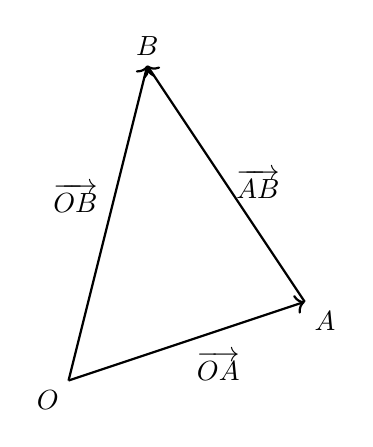
\begin{tikzpicture}
    \coordinate (O) at (0,0);
    \coordinate (A) at (3,1);
    \coordinate (B) at (1,4);

    \draw[->, thick] (O) -- (A) node[midway, below right] {$\overrightarrow{OA}$};
    \draw[->, thick] (A) -- (B) node[midway, right] {$\overrightarrow{AB}$};
    \draw[->, thick] (O) -- (B) node[midway, above left] {$\overrightarrow{OB}$};

    \node at (O) [below left] {$O$};
    \node at (A) [below right] {$A$};
    \node at (B) [above] {$B$};
\end{tikzpicture}
\end{tcolorbox}
\begin{equation}
    \overrightarrow{OB}=\overrightarrow{OA}+\overrightarrow{AB}
\end{equation}
We can also find graphically the result of multiplying a vector by a scalar. Simply scale the
length of the arrow by the scalar quantity but keep the direction the same.
\begin{tcolorbox}
    \centering
\begin{tikzpicture}

    \coordinate (O1) at (0,0); 
    \coordinate (O2) at (0,-2); 
    \coordinate (A) at (3,1);
    \coordinate (B) at (6,2); 
    
    \draw[->, thick, black] (O1) -- node[midway, above] {$\mathbf{a}$} ++ (A) ;
    \draw[->, thick, black] (O2) -- node[midway, below] {$\mathbf{2a}$}++ (B);
\end{tikzpicture}
\end{tcolorbox}
\subsubsection{Scalar and Vector Product}
So far, we have seen that vectors can be added together or multiplied by a scalar. These operations were defined in a way that generalised similar operations with ordinary numbers in such a way that we maintained many of the usual rules of arithmetic. We now want to introduce a concept of multiplication of vectors.
\\
For any two vectors, \textbf{a} and \textbf{b}, through a redefinition of coordinate system,
we can always write \textbf{b} in terms of \textbf{a} component parallel to \textbf{a} and a remaining part perpendicular to \textbf{a}, $\mathbf{b}=\mathbf{b}_{\parallel}+\mathbf{b}_{\perp}$
The final piece of ordinary arithmetic we wish to retain is the concept of
distributivity; that $\lambda(\mu + \nu) = \lambda\mu + \lambda\nu$. With this, we have
\begin{equation}
    \begin{split}
        \mathbf{a}\cdot\mathbf{b}=\mathbf{a}\cdot(\mathbf{b}_{\parallel}+\mathbf{b}_{\perp}) \\
        =\mathbf{a}\cdot\mathbf{b}_{\parallel}\\
        =|\mathbf{a}|\times|\mathbf{b}_{\parallel}|\\
        =|\mathbf{a}|\times|\mathbf{b}|\cos(\theta)  
    \end{split}
\end{equation}
For any vector \textbf{a}, the product of \textbf{a} with itself is
\begin{equation}
    \mathbf{a}\cdot\mathbf{a}=|\mathbf{a}|\times|\mathbf{a}|\cos(\theta)=|\mathbf{a}|^2
\end{equation}
Notice that this gives us a very useful identity for the magnitude of a vector
\begin{equation}
    |\mathbf{a}|=\sqrt{\mathbf{a}\cdot\mathbf{a}}
\end{equation}
In \textbf{Cartesian coordinates} because the dot product of perpendicular coordinates is 0 then
\begin{equation}
    \mathbf{a}\cdot\mathbf{b}=(a_1\mathbf{\hat{i}}+a_2\mathbf{\hat{j}}+a_3\mathbf{\hat{k}})\cdot(b_1\mathbf{\hat{i}}+b_2\mathbf{\hat{j}}+b_3\mathbf{\hat{k}})=(a_1b_1+a_2b_2+a_3b_3)
\end{equation}
We can use the cross product to find the angle between two vectors
\begin{equation}
    \theta=\cos^{-1}\left(\frac{\mathbf{a}\cdot\mathbf{b}}{|\mathbf{a|\times|\mathbf{b}|}}\right)=\cos^{-1}\left(\frac{\mathbf{a}\cdot\mathbf{b}}{\sqrt{(\mathbf{a}\cdot\mathbf{a})(\mathbf{b\cdot\mathbf{b}})}}\right)
\end{equation}
We define the vector product or cross product as
\begin{equation}
    \mathbf{a}\times\mathbf{b}=|\mathbf{a}|\times|\mathbf{b}|\sin(\theta)\mathbf{\hat{n}}
\end{equation}
In Cartesian coordinates the vector product of the same unit vector is 0 and for any two different unit vectors the product can be found using the following rule
\begin{tcolorbox}
\centering
\begin{tikzpicture}
    \draw[->,black]{(0,0) -- (5,0)};
    \draw[->,black]{(5,-2) -- (0,-2)};
\end{tikzpicture}
\end{tcolorbox}
Notice that this product is anti-commutative: $\mathbf{a} \times \mathbf{b} = -\mathbf{b} \times \mathbf{a}$
Using the above basis vector identities, we can write a general formula for the cross product in
Cartesian coordinates:
\begin{equation}
\left(
    \begin{array}{c}
         a_1 \\
         a_2 \\
         a_3
    \end{array}
    \right)
\times
\left(
    \begin{array}{c}
         b_1 \\
         b_2 \\
         b_3
    \end{array}
    \right)
    =
    \left(
    \begin{array}{c}
         a_1 \\
         a_2 \\
         a_3
    \end{array}
    \right)
    \left(
    \begin{array}{c}
         a_2b_3-a_3b_2 \\
         a_3b_1-a_1b_3 \\
         a_1b_2-a_2b_1
    \end{array}
    \right)
\end{equation}
\subsubsection{Vector Calculus}
Suppose we have a vector that depends on some input, such as a time-varying position vector, $\mathbf{r}(t)$. Then varying the input $t$ by some small amount $\delta t$ will change the vector by some corresponding small amount.

\begin{equation}
\delta \mathbf{r}(t) = \mathbf{r}(t + \delta t) - \mathbf{r}(t). \quad (4.4)
\end{equation}

Notice that this small change in the output is itself vector-valued. The quantity $\frac{1}{\delta t}$ is a scalar and we know how to multiply vectors by scalars, so the ratio

\begin{equation}
\frac{\delta \mathbf{r}(t)}{\delta t} = \frac{\mathbf{r}(t + \delta t) - \mathbf{r}(t)}{\delta t} \quad (4.5)
\end{equation}

is well defined and gives an estimate of the rate of change (which in this case is the velocity).

As in the scalar case, we can take the limit as $\delta t$ shrinks towards 0, and define the derivative as

\begin{equation}
\frac{d\mathbf{r}}{dt} = \lim_{\delta t \to 0} \left( \frac{\mathbf{r}(t + \delta t) - \mathbf{r}(t)}{\delta t} \right). \quad (4.6)
\end{equation}

This looks just like the ordinary derivative, but it is worth emphasising again that the result is a \textbf{vector}. This means that the derivative has both a magnitude and a direction.

Integrating a vector function $\mathbf{F}(t)$ with respect to a scalar $t$ involves integrating each component of the vector separately.
    \begin{equation}
        \int \mathbf{F}(t) \, dt = \left( \int F_x(t) \, dt \right) \mathbf{\hat{i}} + \left( \int F_y(t) \, dt \right) \mathbf{\hat{j}} + \left( \int F_z(t) \, dt \right) \mathbf{\hat{k}}
    \end{equation}
A line integral integrates a vector field $\mathbf{F}$ along a curve $C$ parametrised by $\mathbf{r}(t)$. It represents the work done by $\mathbf{F}$ along $C$.
    \begin{equation}
        \int_C \mathbf{F} \cdot d\mathbf{r} = \int_a^b \mathbf{F}(\mathbf{r}(t)) \cdot \mathbf{r}'(t) \, dt
    \end{equation}
Using a line integral we can calculate the length of a curve or path. Suppose a particle travels along a path defined by the position vector $\mathbf{r}(t)$. Over some short time interval, the distance travelled by the particle is
\begin{equation}
    d\ell=\sqrt{d\mathbf{r}\cdot d\mathbf{r}}
\end{equation}
\begin{equation}
    d\ell=\sqrt{\frac{d\mathbf{r}}{dt}\cdot \frac{d\mathbf{r}}{dt}dtdt}\sqrt{\frac{d\mathbf{r}}{dt}\cdot \frac{d\mathbf{r}}{dt}dtdt}
\end{equation}
\begin{equation}
    \ell=\int d\ell=\int \sqrt{\frac{d\mathbf{r}}{dt}\cdot \frac{d\mathbf{r}}{dt}}dt
\end{equation}
\begin{equation}
    \ell=\int \sqrt{\textbf{v}\cdot \mathbf{v}}dt
\end{equation}
\subsection{Functions}
\subsubsection{Introduction}
A function, $f$, is a map between two sets of objects: the \textbf{domain}, $A$, and the \textbf{codomain}, $B$. For each element $x$ of $A$, there is a unique element $f(x)$ in $B$. We denote the relationship between the function and the sets by $f:A\to B$, and we can show the action of $f$ on a particular element as $f:x\mapsto f(x)$. The sets $A$ and $B$ are part of the definition of the function. Although every element in the domain has associated with it an element of the codomain, the converse is not necessarily true: there can be elements of the codomain to which no element in $A$ are mapped by $f$. The set of elements that \textbf{are} mapped to is called the \textbf{range} of the function. The value input to a function is often called the \textbf{argument}, while \textbf{value} is generally reserved for the output.

Given functions $f:A\to B$ and $g:B\to C$, we can define the composite function $g\circ f:A\to C$ as

\begin{equation}
(g\circ f)(x) = g(f(x)) \quad \forall x \in A.
\end{equation}

That is, if $f$ maps $x$ to $y$ and $g$ maps $y$ to $z$, then $g\circ f$ maps $x$ directly to $z$.

\subsubsection{Asymptotes and “Value at Infinity”}
A vertical asymptote is a value that is not contained in the domain of a function, where the value of the function nearby tends towards $\pm\infty$ as the argument tends to the asymptote. Such values are sometimes also referred to as \textbf{singular points} or \textbf{poles}. For example, the function $f:\mathbb{R}\setminus\{0\}\rightarrow\mathbb{R}, f(x)=1/x$ is not defined at $x=0$ but the value of the function near $x=0$ grows without limit. Notice that the value $f$ tends to need not be the same on each side of the asymptote: in this case $\lim_{x\to 0^{+}} f(x) = \infty$, while $\lim_{x\to 0^{-}} f(x) = -\infty$. However, there are also functions for which the two limits are the same, for example $f(x)=1/x^{2}$.

We also often want to know about the value of a function as $x\rightarrow\pm\infty$. Some functions grow without limit for large $x$, but others may gradually tend towards a finite value. In this case, they are said to have a horizontal asymptote. The way to test for this is to manipulate the expression for the function until its behaviour at $\pm\infty$ is clear. 

\subsubsection{Inverse Functions}

One particularly important application of function composition is in defining the inverse function. The inverse of a function $f$ is only defined if $f$ satisfies two properties:

\begin{enumerate}
    \item For every element, $b$, of $B$, there is an element, $a$, of $A$ such that $f(a) = b$,
    \item For any two distinct elements, $x$ and $y$, of $A$, $f(x) \neq f(y)$.
\end{enumerate}

In this case, the function is \textbf{bijective} and we can define the inverse function $f^{-1}:B\to A$ such that $f^{-1}\circ f = I$, where $I:A\to A$ is the identity function ($I(x) = x\ \forall x$). However, even in cases where these properties are not satisfied, we can generally restrict the function such that the inverse of the restriction does exist. If the first property is not satisfied, we can restrict the codomain $\mathcal{B}$ to the range of $f$, $f(A)$. Since every element in $f(A)$ is mapped to by definition, then we can define the inverse function $f^{-1}:f(A)\to A$. If the second property is not satisfied, we can often choose some suitable subset of $A$ as a restricted domain, $D$, for which the property is satisfied.

For example, $f:\mathbb{R}\rightarrow\mathbb{R}$, $f(x) = \sin(x)$ is a valid function but violates both of these properties: its range is $[-1,1] \neq \mathbb{R}$, and it has infinitely many points that map to the same outputs. However, if we consider instead the function $g:[0,\pi]\rightarrow[-1,1], g(x) = \sin(x)$, then both properties are satisfied and we can define $g^{-1}:[-1,1]\rightarrow[0,\pi], g^{-1}(x) = \sin^{-1}(x)$.

In order to compute the inverse function, often we can rearrange the definition $f$ to express its argument in terms of its value.

\subsubsection{Trigonometric Functions}

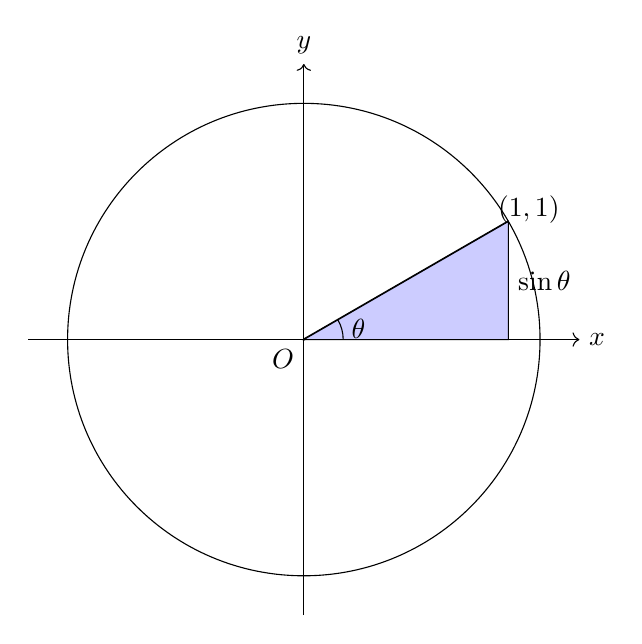
\begin{tikzpicture}
\centering

    \draw (0,0) circle (3cm);

 
    \draw[->] (-3.5,0) -- (3.5,0) node[right] {$x$};
    \draw[->] (0,-3.5) -- (0,3.5) node[above] {$y$};

    
    \def\angle{30} 


    \draw[thick,black] (0,0) -- (\angle:3);

    % Draw the vertical dashed line representing sin(theta)
    \draw[dashed,black] (\angle:3) -- ({3*cos(\angle)},0) node[midway, right] {$\sin\theta$};

    % Fill the section within the dashed line
    \filldraw[fill=blue!20] (0,0) -- ({3*cos(\angle)},0) -- (\angle:3) -- cycle;

    % Label the angle theta
    \draw (0.5,0) arc (0:\angle:0.5) node[midway, right] {$\theta$};

    % Label the point on the circle as (1,1)
    \node at (\angle:3.3) {$(1,1)$};

    % Label the origin
    \node at (0,0) [below left] {$O$};

\end{tikzpicture}


The regular trigonometric functions are defined in terms of a unit circle, $x^{2}+y^{2}=1$. For this reason, they are also sometimes known as the \textbf{circular functions}. By definition, $\sin(\theta)$ is the height of a vertical line from the $x$ axis to the circle that subtends an angle $\theta$, as in Fig. 6.1. The cosine is the horizontal distance of this line from the origin. The other trigonometric functions can also be defined in terms of various projections on this circle, but it is much easier to define them in terms of these first two:

\begin{equation}
\tan(x)=\frac{\sin(x)}{\cos(x)} \quad \cot(x)=\frac{\cos(x)}{\sin(x)}
\end{equation}

\begin{equation}
\sec(x)=\frac{1}{\cos(x)} \quad \csc(x)=\frac{1}{\sin(x)}
\end{equation}

as well as all the usual useful identities:

\begin{equation}
\sin^{2}(x)+\cos^{2}(x)=1
\end{equation}

\begin{equation}
\tan^{2}(x)+1=\sec^{2}(x)
\end{equation}

\begin{equation}
1+\cot^{2}(x)=\csc^{2}(x) \text{ etc.}
\end{equation}

Recall that for a circle of radius $r$, a sector of angle $\theta$ (in radians) has area $r^{2}\theta/2$. Since we are considering the unit circle, another way to define the circular functions is via the area of the sector, rather than the angle. We can define $\sin(\theta)$ as the height of a vertical line from the $x$ axis to a point on the circle that defines a sector with area $\theta/2$, as in Fig. 6.2.

This definition allows for more direct generalisation to another useful set of functions.
We will not prove it here, but the hyperbolic functions can also be defined in terms of the exponential function as

\begin{equation}
\sinh(x) = \frac{e^{x} - e^{-x}}{2} \quad \cosh(x) = \frac{e^{x} + e^{-x}}{2}.
\end{equation}

We can also define the remaining hyperbolic functions in analogy with the circular functions:

\begin{equation}
\tanh(x) = \frac{\sinh(x)}{\cosh(x)} \quad \coth(x) = \frac{\cosh(x)}{\sinh(x)}
\end{equation}

\begin{equation}
\operatorname{sech}(x) = \frac{1}{\cosh(x)} \quad \operatorname{csch}(x) = \frac{1}{\sinh(x)}.
\end{equation}

\subsection{Differentiation}
\subsubsection{Definition}
We define the \textbf{derivative} of $f$ at $x_0$ as 
\begin{equation}
    \frac{df(x_0)}{dx}=\lim_{\delta x\rightarrow 0}\frac{\delta f(x_0)}{\delta x}=\lim_{\delta x\rightarrow 0}\frac{f(x_0+\delta x)}{\delta x}
\end{equation}
\subsection{Integration}



\section{Complex Numbers and Differential Equations}
\subsection{Complex Numbers}
\subsubsection{Introduction to Complex Numbers}
When dealing with quadratic equations with negative discriminants we define ,
\begin{equation}
    \sqrt{ -1 }=i
\end{equation}
A complex number has the form $z=x+iy$ the real and imaginary parts are
\begin{equation}
    x=\mathrm{Re}(z) \quad y=\mathrm{Im}(z)
\end{equation}

Modulus- Distance of $z$ to the origin
\begin{equation}
    |z|=\sqrt{ x^2+y^2 }
\end{equation}
Argument - Angle from real line to the line between the origin and $z$
\begin{equation}
    \arg(z)=\theta=\arctan\left( \frac{y}{x} \right)
\end{equation}
The complex conjugate is defined as a complex number with the same real part but a negative imaginary part
\begin{equation}
    z^{*}=x-iy
\end{equation}
$z$ and $z^{*}$ have the same modulus
\begin{equation}
    |z|=|z^{*}|
\end{equation}
but have different arguments 
\begin{equation}
    \arg(z)=-\arg(z^{*})
\end{equation}
Addition
\begin{equation}
    (x_{1}+iy_{1})+(x_{2}+iy_{2})=(x_{1}+x_{2})+(y_{1}+y_{2})i
\end{equation}
Multiplication
\begin{equation}
    z_{1}z_{2}=(x_{1}+iy_{1})+(x_{2}+iy_{2})=x_{1}x_{2}+ix_{1}y_{2}+ix_{2}y_{2}+y_{1}y_{2}=x_{1}x_{2}+y_{1}y_{2}+i(x_{1}y_{2}+y_{1}x_{2})
\end{equation}


Multiplication with the conjugate
\begin{equation}
zz^{*}=x^2-ixy+ixy+y^2=x^2+y^2=|z|
\end{equation}
Division
\begin{equation}
    \frac{x_{1}+iy_{1}}{x_{2}+iy_{2}}=\frac{x_{1}+iy_{1}}{x_{2}+iy_{2}}\times\frac{x_{1}-iy_{1}}{x_{2}-iy_{2}}=\frac{x_{1}x_{2}+y_{1}y_{2}+i(x_{2}y_{1}-x_{1}y_{2})}{x^2+y^2}
\end{equation}
\subsubsection{Polar Form}
Instead of describing a complex number, $z$, in Cartesian coordinates we can instead represent in $r$ and $\theta$ where,
\begin{equation}
    r=|z| \quad \theta=\arg(z)
\end{equation}
Euler's formula:
\begin{equation}
    re^{i\theta}=r(\cos \theta+i\sin \theta)
\end{equation}
We can use arithmetic for these forms of complex numbers
\begin{equation}
    z_{1}z_{2}=r_{1}e^{i\theta_{1}}r_{2}e^{i\theta_{2}}=r_{1}r_{2}e^{i(\theta_{1}+\theta_{2})}
\end{equation}
\begin{equation}
    \frac{z_{1}}{z_{2}}=\frac{r_{1}e^{i\theta_{1}}}{r_{2}e^{i\theta_{2}}}=\frac{r_{1}}{r_{2}}e^{i(\theta_{1}-\theta_{2})}
\end{equation}
\begin{equation}
    z^n=(re^{i\theta})^n=r^ne^{in\theta}=r^n(\cos \theta +i\sin \theta)
\end{equation}
The $n^{th}$ roots of a complex number are the solution of the equations 
\begin{equation}
    w=z^{\frac{1}{n}}
\end{equation}
Where there are always $n$ roots
\begin{equation}
    z=re^{i \theta}=re^{\theta+2k\pi} 
\end{equation}
For any integer $k$
\begin{equation}
    w_{k}=z^{1/n}=r^{\frac{1}{n}}e^{\frac{i(\theta+2k\pi)}{n}}
\end{equation}

\end{document}